\section{Visión Artificial} \label{sect:Vision_Artificial}

Una manera de obtener información del ambiente es con la visión artificial. Esta consiste en usar un dispositivo (cámara) que
capta el espectro electromagnético y produce una imagen. La representación de la imagen se almacena como una matriz de píxeles,
cada píxel es un elemento que guarda información de una región en el espacio captado. Si se usa una cámara de luz, la información
de cada píxel será el color. \cite{AiRobotics}  

Por lo general luego de obtener una imagen se requiere extraer información de ella, por lo cual se han desarrollado diferentes
algoritmos que ayudan en esta tarea. Existen varios algoritmos que se dedican a la transformación de las imágenes para reducir
ruidos, compensar problemas de iluminación, extraer formas, identificar objetos, entre otros. En esta sección se describen dos
de las técnicas de transformación para reducir el ruido basadas en la dilatación y erosión de la imagen. 

\subsection{Filtros }
El filtrado de imágenes es una técnica para la transformación de imágenes, que consiste en destacar  sus características más relevantes en base a un propósito en particular. 

Generalmente en la tarea de extracción de información de una imagen se utilizan filtros para descartar zonas o características que no son importantes para el patrón deseado y para determinar el área deseada ya sea por patrones de forma o color.

En la investigación, los algoritmos de filtrado aplicados a las imágenes fueron: Clausura Morfológica y Apertura Morfológica, filtros que aplican las técnicas de erosión y dilatación a las imágenes.

\subsection{Transformaciones Morfológicas}
Las transformaciones morfológicas básicas son llamadas dilatación y erosión, se utilizan en 
amplia variedad de contextos como la eliminación del ruido, aislamiento de elementos individuales y elementos de unión dispares
en en una imagen.\cite{BookOpenCv}

\subsubsection{Dilatación}
La dilatación es una convulsión de alguna imagen (o región de una imagen) , que llamaremos A, con un núcleo que llamaremos B,
el núcleo que puede ser de cualquier forma o tamaño, tiene un solo punto de anclaje definido. Muy  a menudo, el núcleo es un
pequeño cuadrado o disco sólido con el punto de anclaje en el centro. El núcleo puede ser pensado como una plantilla  o
mascarilla, y su efecto es que para la dilatación de un operador de máximo local sobre la imagen, se calcula el valor de píxel
máximo común a B y reemplazamos el píxel de la imagen en el punto de anclaje con ese valor máximo. Esto causa regiones brillantes
dentro de una imagen y la hacen crecer. Este crecimiento es el origen del término \" operador de dilatación". \cite{BookOpenCv}

\begin{figure}[hbtp]

\centering
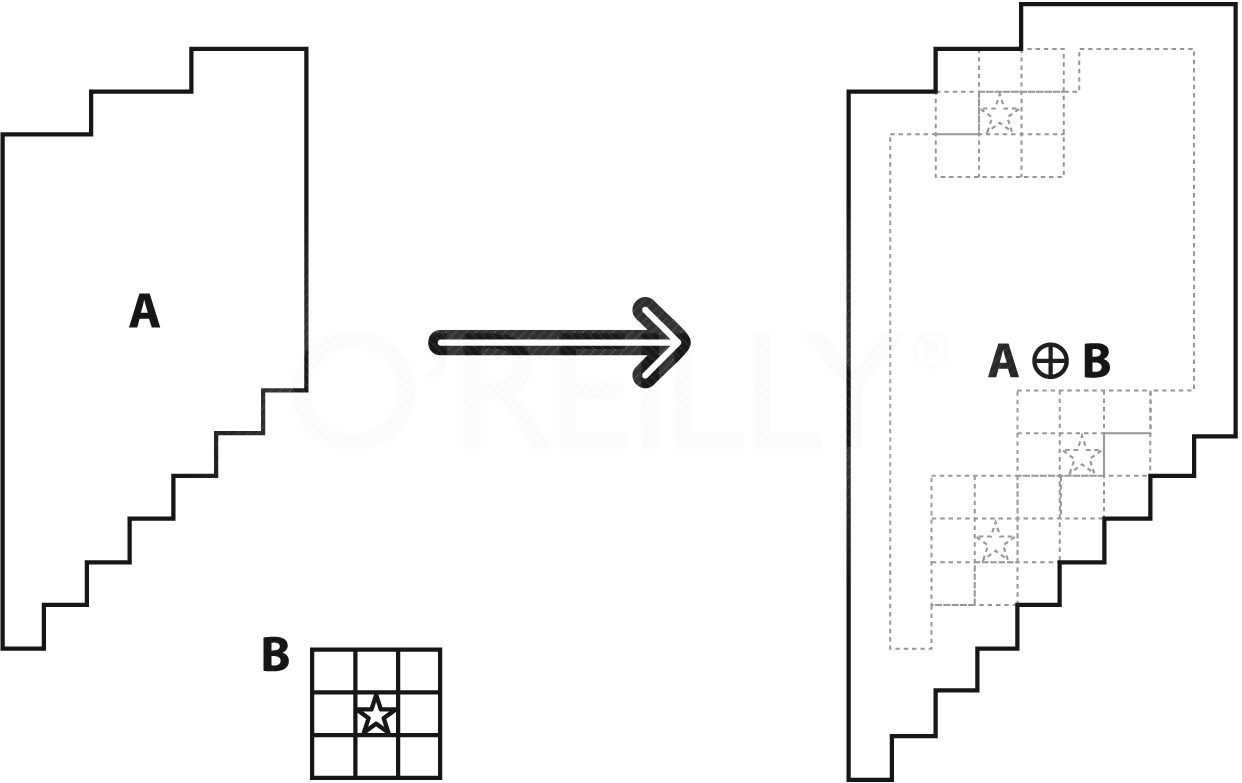
\includegraphics[scale=0.3]{imagenes/erosion-model.png}
\caption{Dilatación}
\end{figure}
\begin{figure}[hbtp]
\label{fig:erosion}
\centering
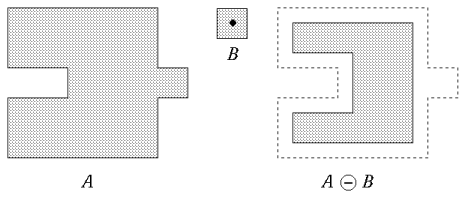
\includegraphics[scale=1]{imagenes/erosion.png}
\caption{Erosión}
\end{figure}


\subsubsection{Erosión}
La erosión es la operación inversa a la dilatación. Esta acción del operador es equivalente a la erosión el cálculo de un mínimo local sobre el área del núcleo. La erosión genera una nueva imagen desde la original, utilizando el siguiente algoritmo: como el
núcleo B es analizado sobre la imagen, se calcula el mínimo valor del píxel superpuesto por B y se reemplaza el píxel de la imagen con un punto de anclaje de valor mínimo. \cite{BookOpenCv}
Vease en la figura \ref{fig:erosion}

